\documentclass[12pt,letterpaper]{article}
\usepackage[margin=1in]{geometry}
\usepackage{mathptmx}
\usepackage{amsmath}
\usepackage{graphicx}
\usepackage{booktabs}
\usepackage{xcolor}
\usepackage{siunitx}
\usepackage[hidelinks]{hyperref}
\usepackage[numbers]{natbib}
\usepackage[font=small,skip=3pt]{caption}
\usepackage{titlesec}
\titleformat{\section}{\centering\normalsize\bfseries}{\thesection.}{0.5em}{\MakeUppercase}
\titleformat{\subsection}{\normalsize\bfseries}{\thesubsection}{0.5em}{}
\titlespacing*{\section}{0pt}{2\baselineskip}{\baselineskip}
\titlespacing*{\subsection}{0pt}{\baselineskip}{0.5\baselineskip}
\usepackage{enumitem}
\setlist{nosep,leftmargin=3em,topsep=\baselineskip}
\setlength{\parindent}{0pt}
\setlength{\emergencystretch}{1.2em}
\setlength{\parskip}{\baselineskip}
\renewcommand{\topfraction}{0.95}
\renewcommand{\bottomfraction}{0.9}
\renewcommand{\textfraction}{0.05}
\renewcommand{\floatpagefraction}{0.85}
\setlength{\textfloatsep}{10pt plus 2pt minus 2pt}
\setlength{\intextsep}{10pt plus 2pt minus 2pt}


\title{}
\date{}

\begin{document}

\begin{center}
{\fontsize{16}{19}\selectfont\bfseries CLOSING THE CONFIGURATION CONSISTENCY
GAP IN A COTS IRIG-106 PCM TELEMETRY SYSTEM\par}
\vspace{2\baselineskip}
{\fontsize{14}{17}\selectfont\bfseries Chiekeziem Udenta, Mason Joyner,
Dominique Stewart\par}
\vspace{0.6\baselineskip}
{\fontsize{14}{17}\selectfont\bfseries Student Paper Advisor: Dr.\ Oluwatobi Busari\par}
{\fontsize{12}{14}\selectfont\bfseries Morgan State University, Baltimore, MD
\\ Rochester Institute of Technology, Rochester, NY\par}
\vspace{4\baselineskip}
\end{center}
\begin{abstract}
This paper describes the design, configuration, and staged verification of
an IRIG-106 Chapter~4 PCM telemetry system for a student-built
liquid-propellant rocket, integrating a twelve-sensor suite through a
Curtiss-Wright KAM-500 chassis, an S-band PCM/FM downlink, and a Lumistar
LS28 ground segment. We argue that in modern COTS telemetry the dominant
integration risk has migrated from hardware to configuration consistency
between the transmit-side frame definition and the ground-side parameter
database, and we demonstrate this failure mode and its mitigation
experimentally. Verification results include over-the-air link
characterization to 120.6~dB equivalent path loss with zero bit errors,
temperature channels verified at the ice point to better than
0.6~\si{\celsius}, and a uniform pressure noise floor of 0.008\% of full
scale through the complete acquisition--transmission--decommutation chain.
An airborne reconfiguration transmitted against a stale ground file pair
--- invisible to receiver lock and frame synchronization --- was flagged
by a frame-embedded counter check on the first frame, with zero false
passes thereafter, while the onboard recorder supplied every frame lost
during a 13.4~s transmitter outage, sample-exact against the downlink.
Configuration consistency, we conclude, is a property to be verified in
the bitstream, not assumed from the toolchain.
\end{abstract}

\noindent\textbf{Key Words:} PCM telemetry; IRIG-106; configuration
management; verification; sounding rocket

\section{Introduction}


The students in Morgan State University's Rocket Propulsion Lab are tackling the complex and intricate task of designing a liquid-propellant rocket to reach an apogee of 50,000ft. Our design calls for utilizing a mixture of RP-1 and liquid oxygen as the propellant pair. Designing a telemetry system that successfully downlinks and collects our high-dynamic data was imperative for live data visualization. Telemetry links trade data rate against robustness: ISRO's Pisharoty
radiosonde pairs low-rate FSK with Reed--Solomon coding~\cite{divya2014},
while NPS's Adamos avionics bay uses a 915~MHz LoRa transceiver, trading
standards compliance for cost~\cite{adamos2021}. This system occupies a
third point --- an IRIG-106 Chapter~4 PCM stream~\cite{irig106} over
S-band PCM/FM --- because two video channels, four pressure ranges, and
GNSS data beyond civilian receiver limits exceed what low-throughput
links carry, and the standard provides interoperability with established
range equipment.

Standards compliance does not eliminate integration risk; it relocates
it. Four decades of hand-built PCM encoders realized frame structures in
programmable logic, verified at the level of
wiring~\cite{rochefort1991,salib2024}; in a modern COTS implementation
the frame definition is compiled in a vendor environment, and the risk
moves to file consistency: the compiled frame definition and the exported
ground-side parameter database must agree exactly, or an error propagates
through an entire dataset as plausible but wrong engineering values ---
in the worst documented case, recovering a mismatched Chapter~4 recording
required manual, hex-level reconstruction~\cite{rettig2017}. This paper
treats configuration consistency as the system's central engineering
risk, demonstrates the failure mode experimentally, and reports a staged
pre-flight verification campaign.

Ground-side reception carries its own trade-offs: larger ranges combat
fades with multiple separated antennas recombined by best-source
selection~\cite{bastie2022} or by digitizing at the antenna into
all-digital multi-channel receivers~\cite{bastie2024}. A single DRSM
receiver and antenna pair suffices for one test article, but our
dual-channel data (\S\ref{sec:results}) already exhibits the
decorrelated fading that motivates source selection at range
scale.

Section~\ref{sec:architecture} describes the architecture,
Section~\ref{sec:frame} the frame design, Section~\ref{sec:methodology}
the verification methodology, Section~\ref{sec:results} the results, and
Section~\ref{sec:lessons} the lessons learned.

\section{System Architecture}\label{sec:architecture}

\subsection{Sensor Suite and Acquisition Mapping}

\begin{table}[htbp]
  \centering
  \caption{Sensor suite and acquisition mapping.}
  \label{tab:sensors}
  \footnotesize
  \begin{tabular}{@{}p{3.4cm}cp{4.8cm}p{4.6cm}@{}}
    \toprule
    Sensor & Qty & Measurement & Acquisition card \\
    \midrule
    RV-CAM HD19 & 2 & Video (H.264 encoded) & 2$\times$ KAD/VID/106 \\
    UNIK 5000 & 4 & Pressure: 350/700/1000/5000 psi FS & KAD/ADC/134 \\
    Omega KMQSS-062U-6 & 3 & Temperature (type K) & KAD/TDC/102 \\
    Trans Cal SSD120(XX)N & 1 & Barometric altitude, RS-232 & KAD/UBM/105 \\
    NovaTel PwrPak7 & 1 & GNSS position/velocity/time & KAM/TCG/105 (+UBM/105) \\
    Multitronix Mx210 & 1 & Recovery altimeter & Independent RF link (own TX/ground RX) \\
    \bottomrule
  \end{tabular}
\end{table}

Three integration decisions merit discussion. First, the PwrPak7 is an
\emph{external} GNSS receiver: civilian receivers cease reporting beyond
the legacy CoCom thresholds (${\approx}$515~m/s and 18~km, carried
forward in the Wassenaar list and ITAR
Category~XV~\cite{wassenaar,itar}), whereas the PwrPak7 measures
continuously to at least 711~m/s and supports a higher output rate than
the TCG/105's onboard receiver. Second, GNSS serial data is routed
through the KAD/UBM/105 in addition to the TCG/105, raising the
position/velocity update rate from 1 to 10~Hz.

The system architecture is shown in Figure~\ref{fig:architecture}. All
acquisition cards reside in a KAM/CHS/13U chassis; a KAD/BCU/101
serves as backplane controller and IRIG-106 Chapter~4 PCM encoder, and a
KAM/MEM/113 logs the full acquired stream to CompactFlash as a recovery
record independent of the RF downlink.

\begin{figure}[htbp]
  \centering
  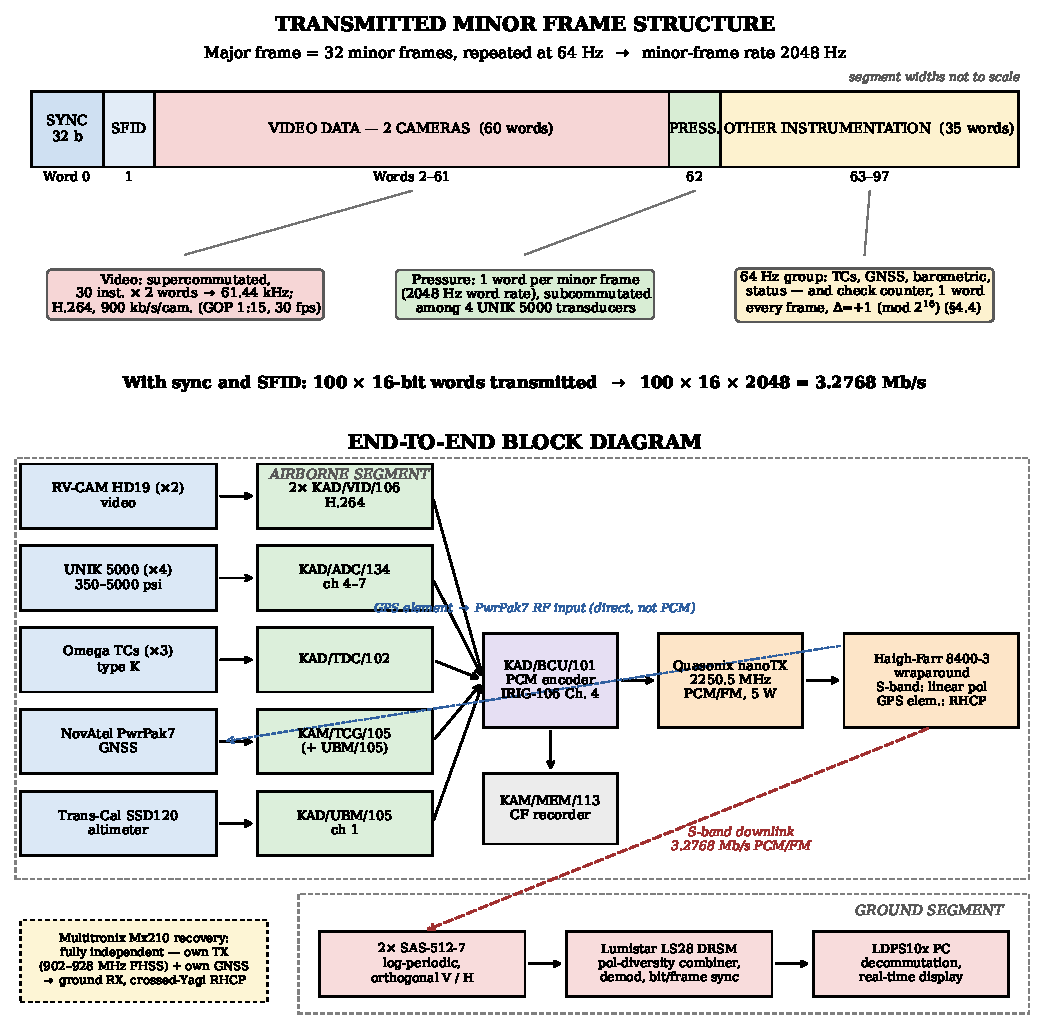
\includegraphics[width=0.94\textwidth]{figs/fig_system_overview.pdf}
  \caption{End-to-end telemetry system: transmitted minor-frame structure
  and parameter allocation (top), and hardware block diagram from sensors
  through PCM encoding, RF transmission, and ground decommutation
  (bottom).}
  \label{fig:architecture}\label{fig:frame}
\end{figure}


\subsection{RF Link}

The PCM baseband stream from the BCU/101 drives a Quasonix nanoTX
transmitter (2200.5--2394.5~MHz, 5~W, heat-sink mounted), configured at
2250.5~MHz with PCM/FM at 3.2768~Mb/s --- the chassis outputs only PCM/FM
without additional modulation hardware. The output feeds a Haigh-Farr
7-inch wraparound antenna (P/N~8400-3) whose S-band element radiates the
downlink; a separate RHCP element receives GPS for the PwrPak7.
Calibrated cuts of the flight unit (S/N~0876, at 2.21, 2.2525, and
2.295~GHz) establish the S-band element is \emph{linearly} polarized,
${\approx}$0 to $+5$~dBi over broad sectors with $-25$ to $-30$~dB
cut-plane nulls (pattern data on file); vehicle roll therefore rotates
the transmitted polarization relative to any fixed ground aperture, with
consequences addressed in \S2.3. The 3.2768~Mb/s stream is dominated by
video (60 of 100 transmitted words); occupied RF bandwidth is not
reported here.

\subsection{Ground Segment}

The ground station is a Lumistar LS28 DRSM --- a dual-channel receiver
performing demodulation, bit synchronization, and onboard IRIG-106 frame
synchronization and decommutation --- feeding a PC where the LDPS10x
suite maps the stream to engineering parameters using a hardware
interface file and parameter database exported from DAS Studio; frame
lock is keyed to the sync word, with the SFID tracking subcommutation
pages.

The flight ground antennas are the SAS-512-7 log-periodic antennas used
throughout the test campaign, with receive antenna gain identified as the
primary area for future improvement. As directional apertures they must be
pointed along the flight path --- boresight tracking of the trajectory is
an operational task of the ground crew. Because the airborne S-band element
is linearly polarized (\S2.2) and the vehicle rolls in flight, the
transmitted polarization rotates continuously relative to the fixed linear
receive apertures, and the resulting roll fades must be absorbed by margin
and diversity. The two log-periodics are therefore mounted orthogonally --- one
vertical, one horizontal --- with the receiver in polarization-diversity
combined mode (LS-28 pre-detection optimal-ratio combiner, ${>}2.6$~dB
S/N improvement near threshold). Between orthogonal apertures roll fades
are anti-correlated by construction: linear transmission at angle
$\theta$ couples as $\cos^2\theta$ and $\sin^2\theta$ respectively,
so the combined response $\propto \cos^2\theta + \sin^2\theta = 1$
is roll-invariant in the ideal case --- the dominant flight-specific fade
mechanism converted to steady combined signal at zero hardware
cost.

The receiver threshold is estimated from datasheet parameters, as the
LS-28-DRSM specifies no single sensitivity figure: a 3--4~dB noise figure
near threshold, an IF bandwidth auto-selected by cascaded SAW and FIR
filtering to match the 3.2768~Mb/s PCM/FM waveform
(${\approx}3.3$~MHz), and a multi-symbol PCM/FM threshold of
${\approx}9$--10~dB $E_b/N_0$ give an estimated sensitivity of
${\approx}{-95}$~dBm. Against the 30~dB fade-margin criterion of
Table~\ref{tab:matrix}, the flight condition would require
${\approx}25$~dBi of aligned linear receive gain; the 6.5~dBi
log-periodics instead provide a predicted ${\approx}12$~dB --- a
documented shortfall accepted for this flight and mitigated by diversity
combining, the onboard MEM/113 record, and the independent Mx210 link,
with a higher-gain aperture as the improvement path.

\section{Telemetry Frame Design}\label{sec:frame}

The telemetry stream is transmitted at 3.2768~Mb/s using 16-bit PCM words and
is organized into 98-word minor frames, with 32 minor frames forming a major
frame that repeats at 64~Hz. Each minor frame begins with a synchronization
word followed by a Subframe Identification (SFID) word, allowing the ground
station to establish frame synchronization and identify the current minor
frame within the major frame sequence. The minor-frame rate is therefore
\(32 \times 64 = 2048\) frames per second, and the stated bit rate is
internally consistent with a 100-word transmitted minor frame:
\(100~\text{words} \times 16~\text{bits} \times 2048~\text{s}^{-1} =
3.2768\)~Mb/s --- the 32-bit frame synchronization pattern and the 16-bit
SFID bringing the 98-word frame to its 100-word transmitted total. Captured TMoIP packets corroborate this independently: 232-byte payloads
decompose as $8 + 24 + 200$ bytes --- exactly the 100 sixteen-bit
transmitted words, one packet per minor frame.

The frame map is shown in the top panel of Figure~\ref{fig:frame}. The majority of each
minor frame carries two supercommutated video channels: 30 instances per minor frame (60 words), grouped by DAS
Studio~3 Burst Placement into uniformly repeated bursts, for an
effective video update rate of 61.44~kHz. The corresponding transport
allocation is 983.04~kb/s per camera, carrying the VID/106's
constant-bit-rate H.264 output (900~kb/s per camera, 30~frames/s NTSC,
GOP ratio 1:15). A single word per minor frame (word~62, 2048~Hz word
rate) is subcommutated among the pressure sensors --- the verification
captures of \S\ref{sec:res-chan}, exercising one sensor per run,
accordingly observed the full word rate on each channel --- and the
remaining words carry GNSS, thermocouple, barometric, and status data at
the 64~Hz major-frame rate.

\section{Verification Methodology}\label{sec:methodology}

Verification proceeds in stages, each layer trusted before the next
depends on it: link characterization, then end-to-end sensor-chain
verification through the link, then configuration fault injection, then
dropout and recovery. Table~\ref{tab:matrix} states each pass criterion in
advance and summarizes results.

\begin{table}[htbp]
  \centering
  \caption{Verification matrix with results to date.}
  \label{tab:matrix}
  \footnotesize
  \begin{tabular}{p{3.2cm}p{3.4cm}p{3.6cm}p{4.2cm}}
    \toprule
    Requirement & Test & Pass criterion & Result to date \\
    \midrule
    Closed link at 9.5~mi slant range with fade margin &
    Range-equivalent attenuation sweep (\S\ref{sec:threshold}) &
    Measured threshold + 30~dB margin at 123.2~dB path &
    Zero BER to 120.6~dB EPL; ${\approx}12$~dB predicted margin --- documented shortfall (\S\ref{sec:res-link}) \\
    Accurate temperature reconstruction &
    End-to-end TC calibration (\S\ref{sec:endtoend}) &
    $\le$1~\si{\celsius} mean error vs reference &
    Ice-point mean error $\le$0.6~\si{\celsius}, $\sigma \le$0.51~\si{\celsius} (RX) (\S\ref{sec:res-chan}) \\
    Accurate pressure reconstruction &
    End-to-end PT verification (\S\ref{sec:endtoend}) &
    $\le$0.5\% FS vs reference &
    Noise $\approx$0.008\% FS all channels; accuracy reference-limited (\S\ref{sec:res-chan}) \\
    Configuration mismatch is detectable &
    Fault injection + test word (\S\ref{sec:fault}) &
    Corrupted database flagged by test-word check before data use &
    Demonstrated: check failed on first frame under stale map; zero false passes over 111~s (\S\ref{sec:res-fault}) \\
    Data survives RF dropout &
    Forced loss of lock + MEM/113 recovery (\S\ref{sec:dropout}) &
    Reacquisition $\le$ one H.264 keyframe interval (0.533~s at GOP 1:15, 30~fps); zero-gap merged record &
    Reacq.\ ${\le}0.09$~s, 27/27; 854-frame fill demonstrated, 99.6\% sample-exact; timestamp merge pending (\S\ref{sec:res-reacq}) \\
    \bottomrule
  \end{tabular}
\end{table}

\subsection{Link Budget and Range-Equivalent Testing}\label{sec:linkbudget}

At the design slant range of 9.5~mi (15.3~km) and 2.25~GHz, free-space
path loss is 123.2~dB. With +35~dBm EIRP (5~W, $-1$~dB insertion loss,
$-1$~dBi typical wraparound gain), matched linear polarizations in the
ground-test geometry, and 1.5~dB receive cable loss, received power with
a 6.5~dBi log-periodic is $-83.2$~dBm --- ${\approx}12$~dB above the
${\approx}{-95}$~dBm derived threshold of \S2.3 and short of the 30~dB
fade-margin criterion of Table~\ref{tab:matrix}, sized against the
measured 11--12~dB ground-test fading, roll-induced polarization
rotation, and attitude nulls. This documented shortfall motivates the
diversity-combining, onboard-recording, and independent-recovery
mitigations of \S2.1 and \S2.3.

Because free-space loss scales as $20\log_{10}(d)$, a fixed attenuator
maps short physical separations to flight-representative equivalent path
loss (EPL): with 40~dB pads, the 113.7~m maximum test separation
reproduces EPL 120.6~dB, i.e.\ ${\approx}$11.4~km of free-space range
--- 74\% of the mission slant range in path-loss terms --- on a 120~m
outdoor path.

\subsection{Receiver Threshold Characterization}\label{sec:threshold}

The RF link is characterized by sweeping equivalent path loss while
logging the LS28 AGC-derived RSSI, $E_b/N_0$, bit error rate, and lock
status, bounding the margin at the 123.2~dB flight condition against the
derived threshold of \S2.3. A preliminary 120~m radiated test with a 40~dB
pad (EPL 121.0~dB) lost lock; the subsequent test with corrected antenna
boresight, reported in \S\ref{sec:res-link}, held lock over the full
sweep.

\subsection{End-to-End Sensor Chain Verification (Temperature and Pressure)}\label{sec:endtoend}

Each thermocouple channel is verified against an ice-point bath and each
pressure channel against a pressurized tank held at a steady reference,
with values read at the LDPS10x display through the complete
sensor-to-engineering-unit chain, and transmit-side values logged
concurrently in IADS; reported per channel: plateau mean, standard
deviation, quantization step, and timing integrity.

Two reference limitations are acknowledged. The ice point is absolute by
physics, but the tank gauge carries lower rated accuracy than the UNIK
5000 transducers, so pressure results are framed as precision and
chain-fidelity measurements with traceable calibration as future work.
Video, GNSS, and the barometric channel are not yet integrated end-to-end;
their verification follows the same pattern, and the RF-layer results are
channel-agnostic and remain valid as channels are added.

\subsection{Configuration Fault Injection}\label{sec:fault}

Each DAS Studio compile is internally self-consistent: the hardware
interface file and parameter database are generated automatically from
one configuration. The vulnerability is in \emph{deployment}: one
compile yields a chassis programming action and a ground file pair,
performed separately, with no mechanism binding the configuration running
in the chassis to the pair loaded in LDPS. The threat is version skew:
(i)~stale ground files after an airborne recompile; (ii)~the reverse,
chassis reprogramming skipped or failed; (iii)~recordings replayed
against the wrong configuration's files --- this campaign itself used
four coexisting compiles distinguishable only by file discipline;
(iv)~a mixed pair from two compiles; and (v)~post-export hand edits that
silently revert on the next export. Burst placement reflows word
positions algorithmically, so a small edit can relocate many parameters;
each export is again perfect, and the mismatch exists only
\emph{between} versions in use.

One class is closed by the toolchain: LDPS validates the SCS file
against the parameter database structurally (words per minor frame must
match the stream exactly), rejecting a mixed pair~(iv) or
geometry-altering skew at load. Geometry-preserving relocations pass, as
does an internally consistent stale pair (i)--(iii), and hand edits~(v)
postdate the check: the validation enforces pair integrity, not
air-to-ground currency.

The mitigation must therefore travel in the bitstream, the only channel
physically connecting the two deployments, and is implemented without
custom hardware: a chassis-native counter, incrementing once per minor
frame and wrapping at $2^{16}$ (32~s), is supercommutated into every
minor frame. The ground station blindly extracts that word position per
its loaded map and applies one test: $\Delta = +1 \pmod{2^{16}}$
between consecutive frames. Reconstructing the staircase requires gating
exactly the correct 16~bits from exactly the correct slot, so any
placement shift, bit misalignment, or geometry-preserving version skew
breaks the test within a frame or two --- before any science data is
trusted --- while the counter doubles as a dropped-frame odometer,
reading $n$ missed frames as $\Delta = n{+}1$.

The check word's coverage is deliberately bounded, with residual classes
assigned to complementary checks: file-side version identity to a
configuration identifier carried alongside the counter, and conversion or
physical-identity errors --- unreachable by any bitstream self-check ---
to the known-stimulus verification of \S\ref{sec:endtoend} with stimuli
\emph{staggered} across channels, since identical stimuli render a
channel swap invisible. The coverage is disjoint and complete at the cost
of one frame word and a pre-flight procedure.

The check was first prototyped by synthesizing elapsed time from the TCG
time fields, for which the expected sequence is
$\{488, 489\}$~\si{\micro\second} per frame; it produced non-integer
differences (non-atomic latching of the constituent words suspected,
same-frame placement unverified) and wraps at the decimal fields' rollover
(99~cs $+$ 9{,}999~\si{\micro\second}, a one-second period) rather than
$2^{16}$~\si{\micro\second}. The native counter superseded it: the counter
ramp was verified against a new frame and configuration file placing the
counter in every minor frame, and a verification tool confirming both the
integral per-frame increment and the counter word's offset from the SFID
--- a two-point cross-check of the loaded map against the live stream ---
is in progress. The live skew demonstration, and two design refinements
adopted from it, are reported in \S\ref{sec:res-fault}.

\subsection{Dropout, Reacquisition, and Recording Redundancy}\label{sec:dropout}

Loss of signal is forced by disconnecting the SMA feeds between the
receive antennas and the LS28 for controlled dwells while both channels
and the MEM/113 record run. Timing derives from logged instruments rather
than manual observation: RSSI timestamps the physical interruption, lock
flags timestamp detection and reacquisition, and trials span 2--30~s
dwells to test whether recovery depends on outage duration. Reported:
medians and extremes over $N$ events, the ground-data gap per event, and
the merged-record demonstration. The same logs disambiguate the
ground-record gaps of \S\ref{sec:res-chan}: gaps with steady RSSI are
logging stalls, not RF dropouts.

\section{Results}\label{sec:results}

\subsection{Link Characterization and Flight-Condition Margin}\label{sec:res-link}

The receiver characterization varied physical separation from 0 to
113.69~m in 20-ft increments through 40~dB attenuator pads, logging RSSI,
$E_b/N_0$, BER, and lock-loss counts on both channels. RSSI degraded from
approximately $-39$/$-50$~dBm at zero separation to $-79$/$-82$~dBm at
maximum. Fits beyond 20~m give path-loss slopes of $-21.4$ (CH1) and
$-18.3$~dB/decade (CH2) against the free-space $-20$, and received power
at maximum separation agrees with the $-80.6$~dBm link-budget prediction
to 1--2~dB (Figure~\ref{fig:rssi}), confirming the EIRP, gain, and
matched-polarization assumptions of \S\ref{sec:linkbudget}.

\begin{figure}[htbp]
  \centering
  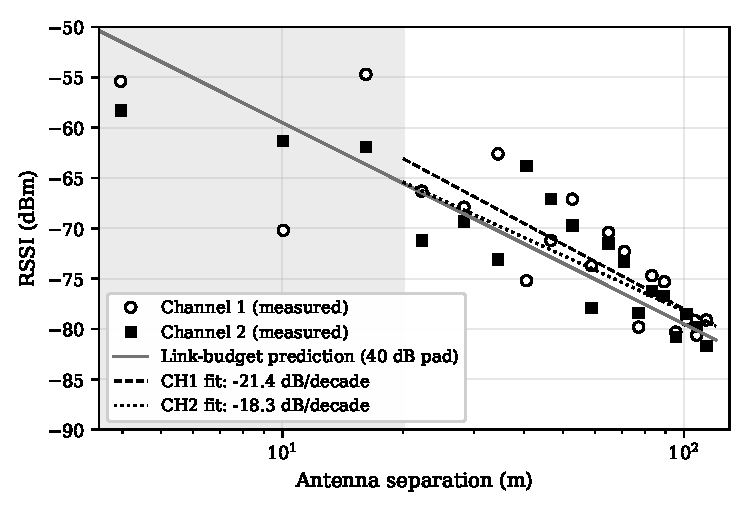
\includegraphics[width=0.48\textwidth]{figs/fig_rssi_vs_distance.pdf}
  \caption{Measured RSSI versus antenna separation for both receiver channels
  with a 40~dB attenuator in line, compared against the link-budget
  prediction. Fitted slopes of $-21.4$ and $-18.3$~dB/decade agree with the
  $-20$~dB/decade free-space model; the shaded region below 20~m is
  excluded from the fit due to near-field and ground-proximity effects.}
  \label{fig:rssi}
\end{figure}

The scatter about the fits is not noise: residuals show 11--12~dB
peak-to-peak quasi-periodic ripple (Figure~\ref{fig:ripple}), consistent
with two-ray ground-reflection fading --- at ${\approx}2$~m antenna
heights the first Fresnel-zone radius at midpath equals the antenna
height. The channels also decorrelate: per-station CH1$-$CH2 differences
reach 11.4~dB with near-zero mean (Figure~\ref{fig:diversity}), so the
two antennas provide genuine spatial diversity --- a small-scale instance
of the decorrelated fading that motivates best-source selection at range
scale~\cite{bastie2022} --- and the initial 120~m failure is explained as
a fade-null-plus-boresight event rather than a threshold crossing.

\begin{figure}[htbp]
  \begin{minipage}[t]{0.49\textwidth}
    \centering
    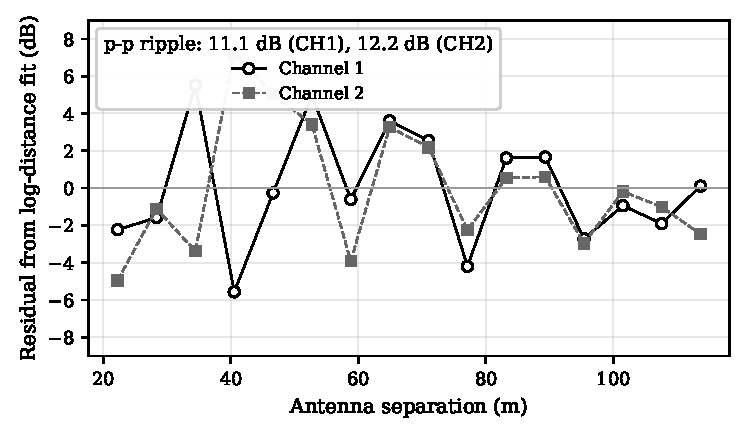
\includegraphics[width=\textwidth]{figs/fig_multipath_ripple.pdf}
    \caption{Residuals from the log-distance fit, showing 11--12~dB
  peak-to-peak ripple consistent with two-ray ground-reflection fading at the
  ${\approx}2$~m test antenna heights.}
    \label{fig:ripple}
  \end{minipage}\hfill
  \begin{minipage}[t]{0.49\textwidth}
    \centering
    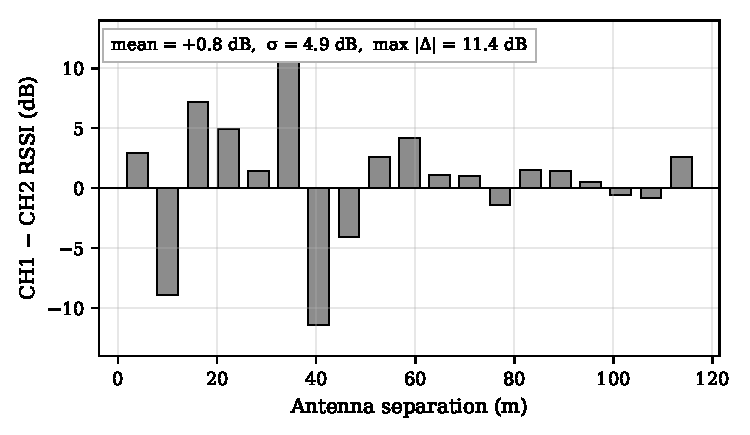
\includegraphics[width=\textwidth]{figs/fig_channel_diversity.pdf}
    \caption{Per-station RSSI difference between the two receive channels.
  Divergence up to 11.4~dB with near-zero mean indicates decorrelated
  multipath fading across the two antennas, providing effective spatial
  diversity.}
    \label{fig:diversity}
  \end{minipage}
\end{figure}



Despite the fading, $E_b/N_0$ held between 15.5 and 21~dB, BER was zero
at every sample, and the near-constant readout across 26~dB of RSSI change
indicates the estimator saturates near its ${\approx}20$~dB ceiling: the
receiver never approached threshold. Lock-loss counts showed no
relationship to distance, implicating transient environmental factors and
possible front-end compression at high signal levels. The dataset
therefore bounds a minimum margin: at EPL 120.6~dB (${\approx}$74\% of
the mission range in path-loss terms), at least 7~dB over a conservative
13~dB single-symbol PCM/FM requirement. The flight condition lies 2.6~dB
beyond the farthest point tested; the characterization stands as a
measured lower bound with the derived $-95$~dBm estimate of \S2.3 as the
working threshold, and flight-specific effects (Doppler, attitude nulls)
justify retaining the onboard MEM/113 recording as non-RF-dependent
redundancy.

\subsection{End-to-End Channel Verification and Timing Integrity}\label{sec:res-chan}

\paragraph{Repetition rates and dropped frames.}
Sample timing was verified independently on both sides: transmit-side
records show exactly 64.000~Hz (temperature) and 2048.00~Hz (pressure)
with zero drops, and receive-side records reproduce the same rates,
confirming the frame structure of Section~\ref{sec:frame} from
measurement. The ground logs are not gap-free --- temperature gaps to
156~ms and one 122-frame pressure gap --- precisely the event class the
MEM/113 merge of \S\ref{sec:dropout} recovers.

\paragraph{Temperature channels at the ice point.}
Table~\ref{tab:temp} reports plateau statistics at the ice-point reference for
the three thermocouple channels on both sides of the link. Receive-side
plateaus (8--13~s dwells) show mean errors of $-0.26$ to $-0.07$~\si{\celsius}
against the 0~\si{\celsius} reference with standard deviations of 0.27--0.51~\si{\celsius},
against a measured quantization step of 25~m\si{\celsius} (the TDC/102 least
significant bit) --- i.e., the observed noise is genuine channel noise of
10--20 counts, not resolution-limited. Transmit-side plateaus were
substantially shorter (0.8--1.8~s) and are reported for completeness; the
temp4 transmit plateau in particular appears not to have fully equilibrated
and its statistics should be treated as indicative only.

\begin{table}[htbp]
  \centering
  \caption{Ice-point plateau statistics, temperature channels (\si{\celsius}).}
  \label{tab:temp}
  \begin{tabular}{llS[table-format=3.0]S[table-format=2.1]S[table-format=-1.3]S[table-format=1.3]}
    \toprule
    Side & Channel & {$n$} & {Dwell (s)} & {Mean} & {$\sigma$} \\
    \midrule
    RX (LDPS) & Temp4 & 593 & 9.3 & -0.157 & 0.350 \\
    RX (LDPS) & Temp5 & 829 & 12.9 & -0.262 & 0.269 \\
    RX (LDPS) & Temp13 & 522 & 8.1 & -0.072 & 0.513 \\
    TX (IADS) & temp4 & 49 & 0.8 & 0.578 & 0.747 \\
    TX (IADS) & temp5 & 112 & 1.7 & 0.368 & 0.246 \\
    TX (IADS) & temp13 & 113 & 1.8 & -0.207 & 0.566 \\
    \bottomrule
  \end{tabular}
\end{table}

The transmit-side capture additionally contains a synchronized anomalous
excursion: exactly 83 samples above 500~\si{\celsius} on all three
channels at once, two pinned at an identical 824.65~\si{\celsius} ---
the common-mode timing and identical clipped values indicate an
electrical or configuration artifact, not a thermal event. These samples
are excluded; recollection was not possible before submission and
root-cause isolation is ongoing work.

\paragraph{Pressure channels at static reference holds.}
Each pressure transducer was held at a steady tank pressure and captured
on both sides (Table~\ref{tab:pressure}). Transmit and receive statistics
agree to 0.014~psi in mean and to the third decimal in standard deviation:
the RF and decommutation chain adds no measurable bias or noise.
Normalizing by full scale collapses all four channels to
${\approx}0.008$\%~FS --- 4.9--5.4 ADC counts (1$\sigma$) --- a
sensor-independent ADC/134 noise floor. The 5000~psi transducer at 2\% of range retained 0.41~psi
resolution, confirming pad-monitoring utility before ignition. As
discussed in \S\ref{sec:endtoend}, absolute accuracy is bounded by the
reference gauge (200~psi full scale, 10~psi graduations, no marked class),
which read ${\approx}100$~psi against the decommutated 100.28~psi for the
one hold recorded --- within half-graduation readability --- with the
other holds standing as precision measurements.

\begin{table}[htbp]
  \centering
  \caption{Static-hold statistics, pressure channels (engineering units, psi).}
  \label{tab:pressure}
  \small
  \begin{tabular}{lS[table-format=3.3]S[table-format=1.3]S[table-format=3.3]S[table-format=1.3]S[table-format=1.4]S[table-format=1.1]}
    \toprule
    Sensor & {TX mean} & {TX $\sigma$} & {RX mean} & {RX $\sigma$} & {$\sigma$, \% FS} & {$\sigma$, counts} \\
    \midrule
    5000 psi & 100.278 & 0.415 & 100.265 & 0.413 & 0.0083 & 5.4 \\
    1000 psi & 73.686 & 0.083 & 73.683 & 0.083 & 0.0083 & 5.4 \\
    700 psi & 93.283 & 0.053 & 93.283 & 0.052 & 0.0076 & 4.9 \\
    350 psi & 91.749 & 0.028 & 91.749 & 0.028 & 0.0080 & 5.2 \\
    \bottomrule
  \end{tabular}
\end{table}

One metadata note: the LDPS export labeled the pressure values ``VDC''
while IADS presented identical numbers as pressure --- an ad hoc raw-data
conversion during setup, retained as an illustration of how readily semantic
metadata diverges between tools once manual conversions enter the chain
(scenario~v of \S\ref{sec:fault}).

\subsection{Configuration-Skew Detection}\label{sec:res-fault}

The version-skew failure mode and its detection were demonstrated live,
in the most realistic direction: a configuration (XidML) omitting the
counter was programmed into the chassis while the ground retained its
previous file pair --- scenario~(i) with the skew airborne. Throughout
the 111~s stale-map period the receiver stayed locked and the SFID cycled
correctly (99.997\% of transitions) --- the silent regime --- and the
check word alone exposed the mismatch: $\Delta = +1$ failed on the very
first frame comparison ($\Delta = 13{,}422$), and over 80{,}171
subsequent comparisons the position formerly carrying the counter passed
by chance in only 0.59\% of isolated frames, never three consecutively
--- a three-frame (1.5~ms) window yields zero false passes. The
correct-pair period passed 99.997\% of 74{,}863 comparisons, its two
exceptions one $\Delta = 32$ event: the odometer registering a 31-frame
loss. Reprogramming the correct configuration restored the staircase
(Figure~\ref{fig:skew}). Two refinements were adopted: relocating the
counter word on every configuration change, and a configuration-number
word per major frame, upgrading detection to identification.

\begin{figure}[htbp]
  \centering
  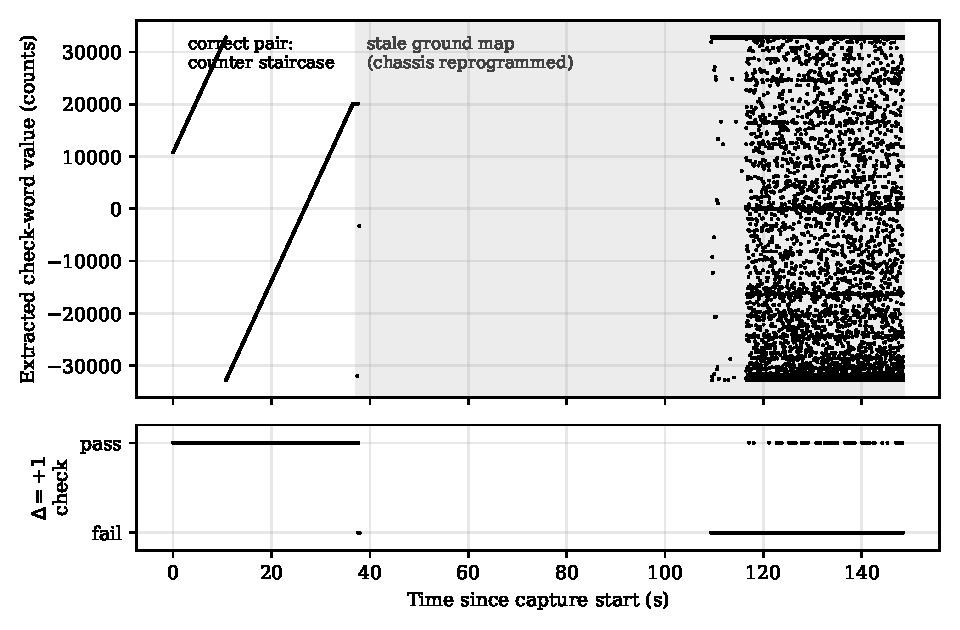
\includegraphics[width=0.5\textwidth]{figs/fig_skew_detect.pdf}
  \caption{Live configuration-skew detection. Extracted check-word value
  (top) and the $\Delta = +1$ test (bottom): the counter staircase under
  the correct file pair, and immediate, sustained check failure after a
  configuration omitting the counter was programmed into the chassis
  against the stale ground map (shaded). Receiver lock and SFID cycling
  remained intact throughout.}
  \label{fig:skew}
\end{figure}

\subsection{Reacquisition Statistics}\label{sec:res-reacq}

The interruption protocol was executed as 27 forced interruptions across
2--30~s nominal dwells (0.5--30.7~s measured), both SMA feeds
disconnected in each event, RSSI falling to the channel noise floors; the
${\pm}0.5$~s channel-to-channel offsets reflect manual handling of two
connectors, so the bound below applies from signal restoration at each
input.

Three results follow: reacquisition is faster than the log resolves
(all 27 events relocked within the same 88.6~ms interval as RSSI
restoration; channel~2 within $-1.5$ to $+0.6$~s of channel~1); recovery
is independent of outage duration from 0.5 to 30.7~s; and carrier and
bit-sync lock recovered together, the locked bit-sync count of
$3.2766$--$3.2782 \times 10^{6}$~counts/s independently confirming the
bit rate.

Figure~\ref{fig:reacq} shows a representative 30~s event. Two limitations
bound these results: the test was conducted at an operating point
(RSSI ${\approx}-79$ to $-81$~dBm, $E_b/N_0 \approx 19$--20~dB)
representative of the longest-path condition of the range characterization
of \S\ref{sec:res-link} (EPL ${\approx}120.6$~dB) --- i.e., near-flight
signal levels, but not near threshold. The transmitter power-cycle case
and the onboard-record continuity result are reported below.

\paragraph{Transmitter power-cycle interruption.}
A transmitter power-cycle --- additionally exercising start-up settling
and cold-oscillator reacquisition --- was performed during a 137.2~s
capture. The downlink lost 13.369~s (855 major frames, corroborated to
1.4\% by the retrieved-frame deficit), bounding the combined off-dwell
and reacquisition. Distinctly from the receive-side case, relock was
followed by a 0.638~s transient dropping 41 major frames at alternating
intervals before the stream settled --- lock declaration precedes clean
data after a cold start.

\paragraph{Onboard-record continuity.}
The MEM/113 record spanning the event provides recoverability: packet
sequence numbers contiguous across the entire 1{,}035~s recording, all
428 packets covering the outage present, and no sequence reset ---
the acquisition unit never power-cycled. Every sample the downlink lost
exists onboard.

\paragraph{Content-aligned merge demonstration.}
\begin{sloppypar}
In the initial session the records differed by 1~d~05:01:26 (acquisition-unit clock versus the
LS-28 time module) and the parameter was recorded at 32~Hz
against a 64~Hz downlink. A repeat session resolved both: with the
onboard stream re-logged at 64~Hz, a second power-cycle (13.369~s, 854
frames, duration reproduced to the millisecond --- the power-off
procedure itself) was captured with a deliberate thermal transient for
identification. Gap-aware time alignment identifies the downlinked
parameter within the onboard record at sample level: 99.60\% of
10{,}341 overlapping samples agree exactly (RMS 1.2 counts), residuals
confined to top-decile slew intervals (to 165~\si{\celsius}/s) where
sub-frame timing skew dominates. The onboard record supplies all 854
missing frames with clean continuity at both edges
(Figure~\ref{fig:merge}); onboard cadence measured 64.000~Hz exactly
with zero sequence breaks. The absolute offset, with ground time read as
UTC, now decomposes to exactly one day plus 1.1~s --- the zone component
resolved, leaving a date-field error and ${\approx}1$~s set error before
a fully timestamp-driven merge, which remains work in progress.
\end{sloppypar}

\begin{figure}[htbp]
  \centering
  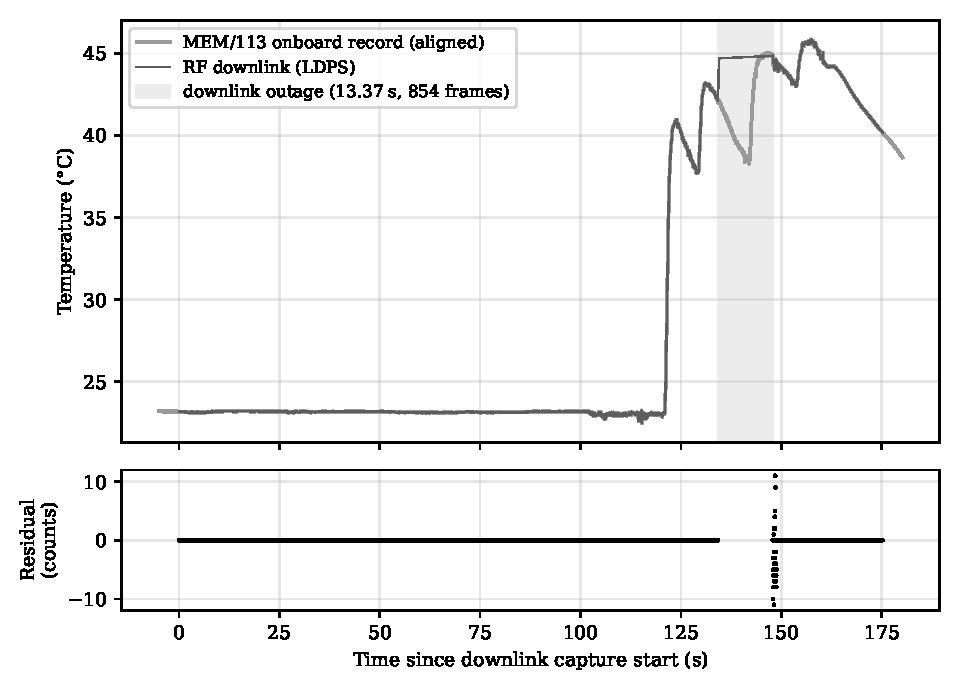
\includegraphics[width=0.5\textwidth]{figs/fig_merge_demo.pdf}
  \caption{Content-aligned merge demonstration. The onboard MEM/113
  record (grey), aligned to the RF downlink (red) by gap-aware
  time alignment of raw counts, supplies all 854 frames lost during the
  13.37~s transmitter power-cycle outage (shaded). Lower panel: per-sample
  residual between the records over the overlap; 99.60\% of samples agree
  exactly.}
  \label{fig:merge}
\end{figure}

\begin{figure}[htbp]
  \centering
  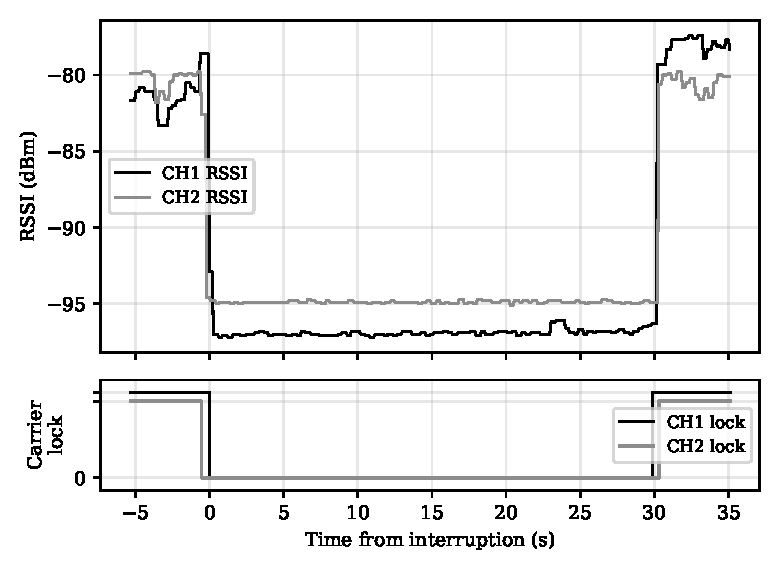
\includegraphics[width=0.48\textwidth]{figs/fig_reacq_event.pdf}
  \caption{Representative 30~s forced interruption: RSSI (top) and carrier
  lock (bottom) for both receiver channels. Lock returns within one 88.6~ms
  log interval of signal restoration.}
  \label{fig:reacq}
\end{figure}

\section{Lessons Learned}\label{sec:lessons}

\begin{itemize}
  \item COTS tooling relocates rather than removes integration risk: the
  failure-sensitive link is file consistency between the compiled frame
  definition and the exported parameter database, with no toolchain check
  of air-to-ground currency --- budget verification effort there, not in
  the hardware.
  \item A fixed attenuator is not a range simulator by itself; it
  multiplies the physical test separation ($10\times$ per 20~dB). Report
  pad value and separation together as equivalent path loss.
  \item At ground-test antenna heights the first Fresnel zone is
  obstructed: expect two-ray fading of 10~dB or more; a fixed-geometry
  pad sweep, not a walk-out, is the instrument for threshold
  measurement.
  \item A single frame word spent on a known counter converts the worst
  silent failure mode into a routine pre-flight check at 1\% of link
  capacity.
  \item Keep recovery-critical functions (the Mx210 deployment altimeter)
  out of the telemetry chain entirely.
  \item Lock declaration is not clean data: after a transmitter power
  cycle, 41 major frames dropped over 0.64~s post-relock; validate the
  first second of post-relock data.
  \item Two undisciplined clocks cannot align two records (ours disagreed
  by 1~d~05:01:26): discipline both ends or align on content, and record
  merge-critical parameters at the downlink rate.
\end{itemize}

\section{Conclusion}

This paper set out from a claim about where the risk lives in a modern
COTS telemetry system: not in the hardware, but in the deployment gap
between the configuration running in the chassis and the file pair loaded
on the ground. The staged campaign bore the claim out at every layer:
path-loss slopes of $-21.4$ and $-18.3$~dB/decade against the free-space
$-20$, received power within 1--2~dB of budget, zero bit errors to
120.6~dB EPL, with the measured 11.4~dB channel decorrelation motivating
the orthogonally polarized diversity configuration adopted for flight;
ice-point mean errors below 0.6~\si{\celsius} and a uniform
${\approx}5$-count (0.008\%~FS) pressure noise floor carried through
the complete chain; relock within one 88.6~ms log interval across 27
interruptions; and an onboard record supplying all 854 frames lost to a
13.4~s transmitter outage, sample-exact against the downlink.

The central demonstration closed the argument. A configuration omitting
the check parameter was programmed into the chassis against a stale
ground map: the receiver stayed locked, the SFID cycled, every parameter
decommutated plausibly --- and the frame-embedded counter failed on the
first frame, with zero measured false passes over 111~s under a
three-frame window. One sixteen-bit word, at 1.0\% of link capacity,
converts the silent failure mode into a pre-flight go/no-go check;
together with the structural validation the ground software performs and
the staggered known-stimulus procedure, the system carries a layered,
experimentally characterized defense across the failure space.

What remains before flight is enumerable: the date-field correction
completing the timestamp-driven merge, automation of the verification
tool, GPS-disciplined outdoor operation, and the remaining channels under
the same verification pattern. The broader conclusion travels beyond this
vehicle: for a student program adopting COTS PCM telemetry, the
architecture arrives correct by construction --- the engineering
substance lies in verifying, continuously, in the bitstream itself, that
what the ground believes about the frame is what the vehicle is actually
transmitting.

\section{Acknowledgments}

The authors gratefully acknowledge Curtiss-Wright, NovAtel, Lumistar, and
Haigh-Farr for hardware and personnel support, and Quasonix for providing
the program's transmitter; Embry-Riddle Aeronautical University, Purdue
University, and Virginia Tech for collaborative assistance; and NASA MSFC,
U.S. Army DEVCOM, Aerojet Rocketdyne, the Aerospace Corporation, and the
Morgan State University Administration, whose funding, initiative, and
sustained commitment made this program possible. Per ITC guidelines, the authors disclose the use of Anthropic's Claude
large language model in preparing this paper; the tool and extent of its
contribution are specified in~\cite{claude2026}.

{\footnotesize
\setlength{\bibsep}{0.5pt plus 0.5pt}
\bibliographystyle{unsrtnat}
\bibliography{references}}

\end{document}
